\chapter{Single Photon Interference And Superposition}

\chapterprecis{Optics Practicum 3} 

\makeoddhead{myheadings}{\emph{Single Photon Interference}}{}{\thepage}
\makeevenhead{myheadings}{\thepage}{}{\emph{Optics Practicum 3}}

\section*{Introduction}

In section 3 of \emph{The Principles of Quantum Mechanics}, in order to develop his notion of "superposition" further, Dirac proposes to describe what happens when a single photon enters an "interferometer." With the use of our equipment, we can carry out this experiment in fact.

Our interferometer makes use of an arrangement of two beam-splitters and two mirrors to separate and then recombine one beam of light. One of the mirrors is fixed, and the other is movable. The latter is very gradually moved so as to change the length of one of the paths by which the light makes its way through the apparatus. This changing of one path length is what will allow interference effects to appear, as light of a single frequency is recombined with itself with different degrees of shift in phase, just as different distances to the screen in double-slit diffraction create an interference pattern. Since the mirror is uniformly advanced by a constant interval and the result of measurement is graphed after each nudge, the interference will manifest itself as a familiar sinusoidal pattern in the output at the detector, oscillating between a maximum intensity and zero, as if two beams of light were being made to constructively and destructively interfere with each other. Dirac's account invites us to think about how the state of a single photon must be described if it, too, is subject to interference. How can a single photon interfere with itself? According to Dirac, "we must now describe the photon as going partly into each of the two components into which the incident beam is split."

%%%% figure: inteferometer %%%%%

\begin{figure}[h]
  \begin{center}
    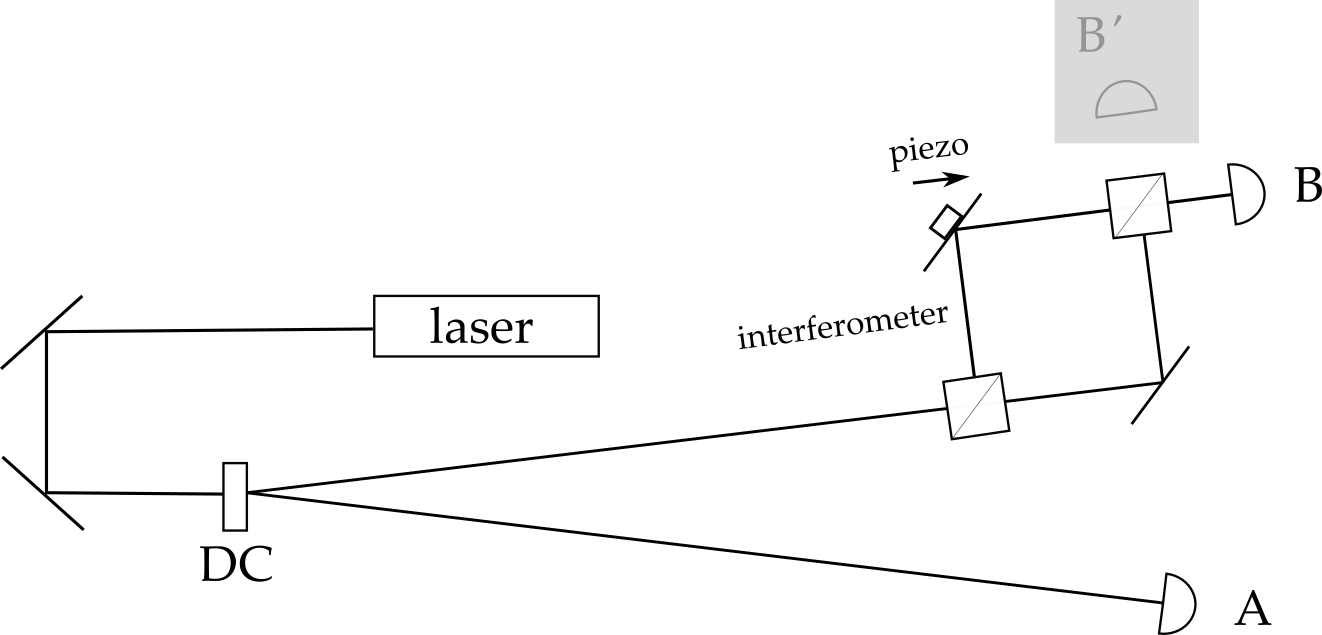
\includegraphics[width=4.40667in,height=2.11667in]{images/14_interference/interference-apparatus.png}
    \captionsetup{width=.75\textwidth}
    \caption*{\emph{Experimental setup for detecting single-photon interference. An optional second detector
    can be set up at $B'$ if desired after the main demonstration is complete.}}
  \end{center}
\end{figure}

\section*{The Singleness of Photons}

For our experiment to be a useful occasion for thinking through this account of superposition, we need to be reasonably sure that there is only one photon at a time in the interferometer.  A brief calculation of how many photons are in the apparatus at a time follows.

If the maximum rate of detection of photons from the laser is 87,500 per second (which, even after painstaking adjustment of the precise positions of all the optical elements, would be on the high end for our equipment), and the detectors register one out of every 10 photons (a conservative estimate, given the efficiency ratings of the detectors, which may be as high as 50\%), then the number of photons coming through per second could be as many as $87,500/0.1$ or $875,000$.  Since the speed of light is $3\times 10^{10}$ centimeters per second, the ``number'' of photons that could be found in each centimeter at any one time is

\[\frac{875,000 \; \text{per sec}}{3 \times 10^{10}\; \text{cm/sec}} = 2.9 \times 10^{-5}. \]

The length of the interferometer will vary slightly each time it is set up, but one of its arms is generally about 20 cm long.  Therefore, the average number of photons in the interferometer at any one time is 

\[2.9 \times 10^{-5} \; \text{per cm} \times 20 \; \text{cm} = 5.8 \times 10^{-4}. \]

Or, since this is a number much less than one, we can say that the \emph{chance} of there being a photon from the laser in the interferometer at any given instant is 0.058\% or about 1 in 1700. The chance that two are present, therefore, is almost 3 million to one. Consequently, we can be reasonably sure that the overwhelming majority ($> 99.9\%$) of photons coming through the interferometer and being registered at the detectors have traveled through it unaccompanied. Any inteference effects they suffer must somehow be due to themselves.

\section*{Collecting Data}

Recall from the last practicum using this equipment that \emph{the overhead lights must not be on} while the sensitive photodiode detectors are on.  Recall also that \emph{safety glasses must be worn} when the blue laser is on.

When the experiment is running, the mirror will move a small distance every tenth of a second and then the photon counters will count how many photons they detect. The computer interface will form a graph of these totals as it records them.

